Cloud computing enables the delivery of numerous computing services, including processing power, data storage, data analytics, networking and software, over the Internet. The demand on scalable and agile services has triggered an ecosystem of cloud computing, in which users can optimize cloud systems by integrating virtualized resources and obtain cost advantage compared to in-house IT infrastructure. In addition, the autoscaling of elastic services automatically allocate computational resources when the production workloads are unpredictable, allowing the system to handle the variable traffic spikes better.

To address the security concern and networking latency, cloud computing has evolved into a stratified system that contains IoT clusters, edge cloud and data centers. In this paradigm, edge cloud serves as the middle layer between IoT devices and data centers that brings the computational power and data storage near the deployment sites in hope of improving round-trip time and bandwidth usage. Thus, in the scenarios like real-time data streaming from sensors or users, edge cloud plays a critical role in timely execution and content delivery. 

Particularly, with the arrival of powerful edge cloud devices, computing tasks that requires significant computational power can now be executed on edge devices. Such capability brings more complex machine learning models that analyzes large amounts of dataset closer to data sources and reduces networking latency. This movement has given rise to "edge-based" machine learning that deploys advanced algorithms such as convolutional neural networks (CNNs) at the edges of the network.

However, as the edge cloud acquires exponential growth in computing power, the processor power dissipation imposes an unprecedented challenge to the entire cloud system. Processors in edge cloud devices can age drastically fast or severely damaged by overheating, even they are protected with operational safeguards such as throttling and automatic shutdown~\cite{ref:overheating}, because of the wide-ranging temperature at the deployment sites of edge cloud. Figure\ref{fig:time_series} depicts the time series of CPU temperature in the edge cloud deployed at the Sedgwick Natural Reserve~\cite{ref:sedgwick} in Santa Barbara County, California. The seasonality and glitches of the time series manifest the fluctuation of ambient temperature causes overheating and potential damage to the edge devices. Such scenario motivates the development of a new effective solution to protect edge cloud from overheating.

\begin{figure}
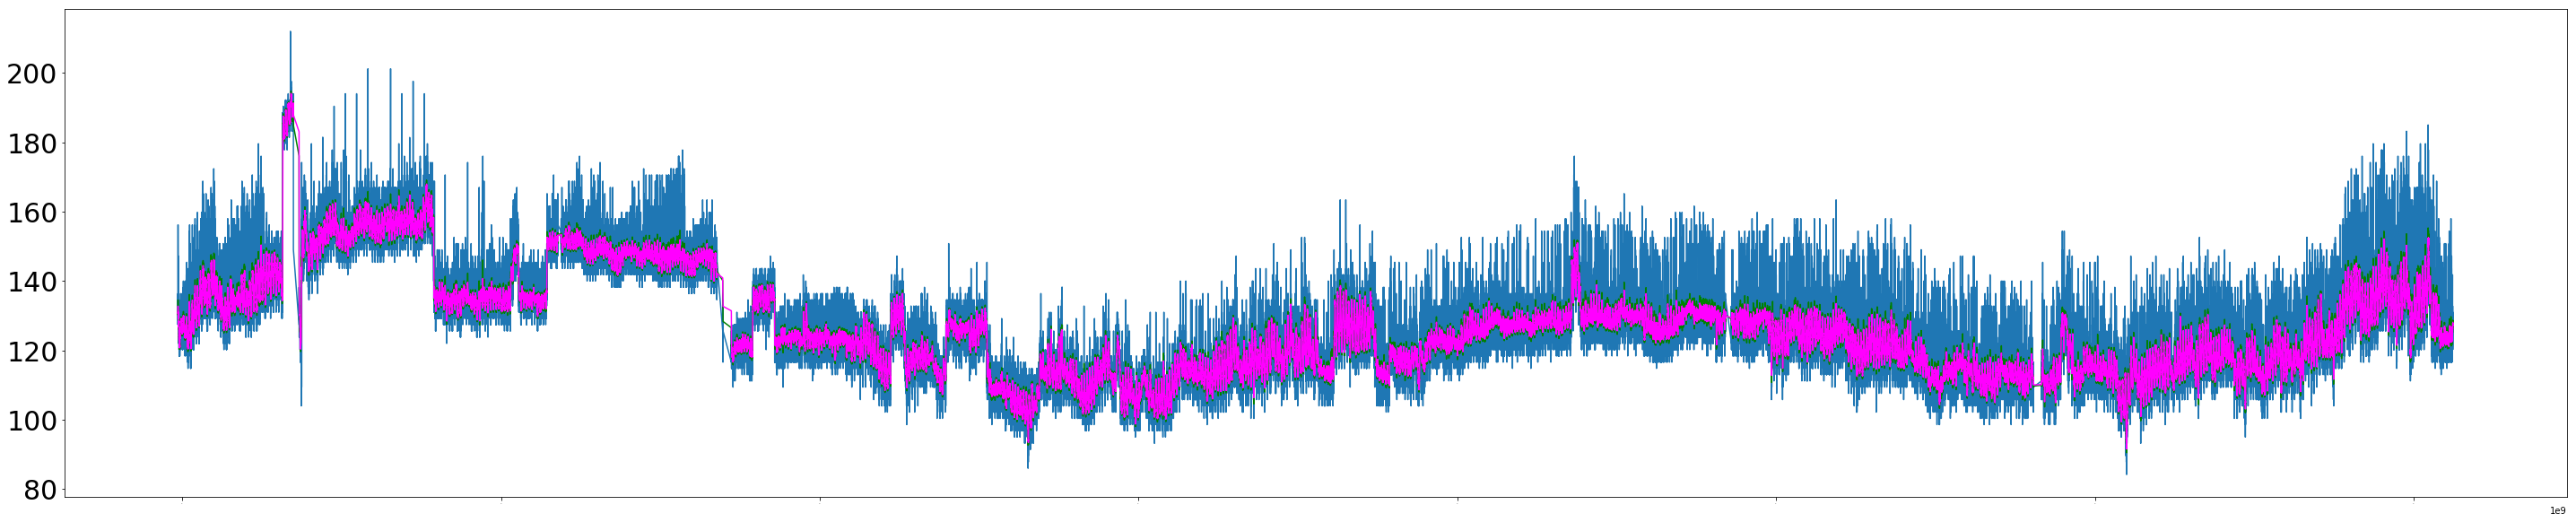
\includegraphics[width=\textwidth]{figures/time_series.png}
\caption{The time series of CPU temperature in the edge cloud deployed at Sedgwick Natural Reserve from Feb. 28th, 2018 to Jun. 3rd, 2020. The x-axis is the epoch time and the y-axis is the CPU temperature in Fahrenheit. } \label{fig:time_series}
\end{figure}

In this work, we propose a heat budget-based scheduling system, \textbf{Sparta}, and investigate its efficacy to control the CPU power dissipation process and prevent CPU temperature from surpassing the preset threshold. In particular, we study the relationship among CPU frequency, temperature, power dissipation and execution pattern, based on which we adopt three modes for Sparta's scheduler. Under the condition that the CPU temperatures are within the threshold, Sparta strives to harness the seasonality of ambient temperature and minimize the execution time of application.

Sparta takes an application, corresponding dataset and a preset temperature threshold as inputs and automatically schedules the workload based on the online sampling temperature data. We use the system to perform a range of machine learning algorithms, including image recognition, natural language processing, decision forest and time series prediction. They comprehensively represent different execution pattern of machine learning application that we utilize in the real-world scenarios.

We build three modes within Sparta's scheduler: \textbf{Annealing} leverages epsilon-greedy strategy to extrapolate the proper CPU frequency in real time; \textbf{AIMD} combines linear growth of CPU frequency when temperature is under threshold with an exponential reduction when it detects any temperature anomaly; \textbf{Hybrid} consolidates Annealing and AIMD modes to overcome their drawbacks and maximizes the efficiency of scheduler. Our results show that Sparta in Hybrid mode speeds up the execution of applications by \textbf{1.16x} and \textbf{1.14x} on average in three thermal environments compared to Annealing and AIMD. In the meantime, Sparta in Hybrid mode has \textbf{94.4\%} of CPU temperature samples remain under the preset threshold on average across all six benchmarks. 

In summary, with this paper, we make the following contributions:

\begin{itemize}
    \item We investigate the relationship between CPU frequency and sampling temperature to precisely model and manage processor power dissipation during execution;
    \vspace{1mm}
    \item We design and implement a heat budget-based scheduling framework that protects edge cloud from overheating and potential damage;
    \vspace{1mm}
    \item We empirically evaluate the efficacy of using Sparta to control CPU temperature and accelerate machine learning applications on six real-world benchmarks in three thermal spectra. 
\end{itemize}

In the following sections, we first present the design and implementation of Sparta (Section~\ref{sec:Sparta}). We then demonstrate our experimental methodology and empirical evaluation of the system by applications in three different thermal environments (Section~\ref{sec:eval}). A body of related work is discussed next (Section~\ref{sec:relate_work}). Finally, we present our conclusions and future work plans.